\section{Implementación del Sistema y Pruebas}

En este capítulo se presenta el entorno técnico en el que se llevó a cabo la implementación del \textit{Nez-Daemon Watcher}, así como las herramientas y procedimientos empleados durante su fase de validación. El propósito es ofrecer una descripción clara de los componentes de hardware y software utilizados, además de documentar las pruebas realizadas para confirmar que el sistema opera conforme a los requerimientos establecidos.

\subsection{Hardware Utilizado}

Para el desarrollo y las pruebas del proyecto se optó por utilizar un equipo de cómputo personal, en lugar de solicitar uno al CINVESTAV. Esta elección respondió principalmente a la necesidad de contar con un entorno de trabajo disponible de manera continua, tanto en la oficina como fuera de ella. El sistema se implementó y evaluó en una computadora portátil HP Victus, cuyo uso permitió mantener un flujo de trabajo estable y replicable durante el proceso de desarrollo.

A continuación se presentan las especificaciones del hardware empleado, con el fin de contextualizar las condiciones bajo las cuales se ejecutaron las pruebas y de proporcionar una referencia para cualquier futura réplica o comparación de resultados:

\begin{itemize}
    \item \textbf{Procesador: Intel Core i5 de 12.ª generación.} Este procesador de múltiples núcleos fue fundamental para ejecutar de manera fluida y simultánea el entorno de desarrollo, el motor de Docker y los múltiples contenedores que simulaban el ecosistema de MictlanX.
    
    \item \textbf{Memoria RAM: 16 GB.} La capacidad de la memoria RAM fue crucial para gestionar la carga de trabajo del sistema. Permitió que el sistema operativo, el entorno de desarrollo, el demonio de Docker y todos los servicios contenedorizados (Peers, Router, SPM) operaran de forma concurrente sin degradar el rendimiento.
    
    \item \textbf{Almacenamiento: 500 GB SSD M.2.} El uso de un disco de estado sólido (SSD) con interfaz M.2 ofreció altas velocidades de lectura y escritura. Esto impactó positivamente en la eficiencia del desarrollo, reduciendo los tiempos de arranque de los contenedores y acelerando las operaciones de entrada/salida del sistema de archivos, un aspecto clave para las pruebas del \textit{Watcher}.
    
    \item \textbf{GPU: NVIDIA GeForce GTX 1650 (4 GB VRAM).} Si bien el servicio \textit{Watcher} no hace un uso intensivo de la unidad de procesamiento gráfico (GPU), su presencia en el equipo de desarrollo asegura la capacidad de ejecutar futuras cargas de trabajo relacionadas con el análisis de datos o el aprendizaje automático, que son casos de uso comunes en la plataforma \textit{Nez}.
\end{itemize}

\begin{figure}[h!]
    \centering
    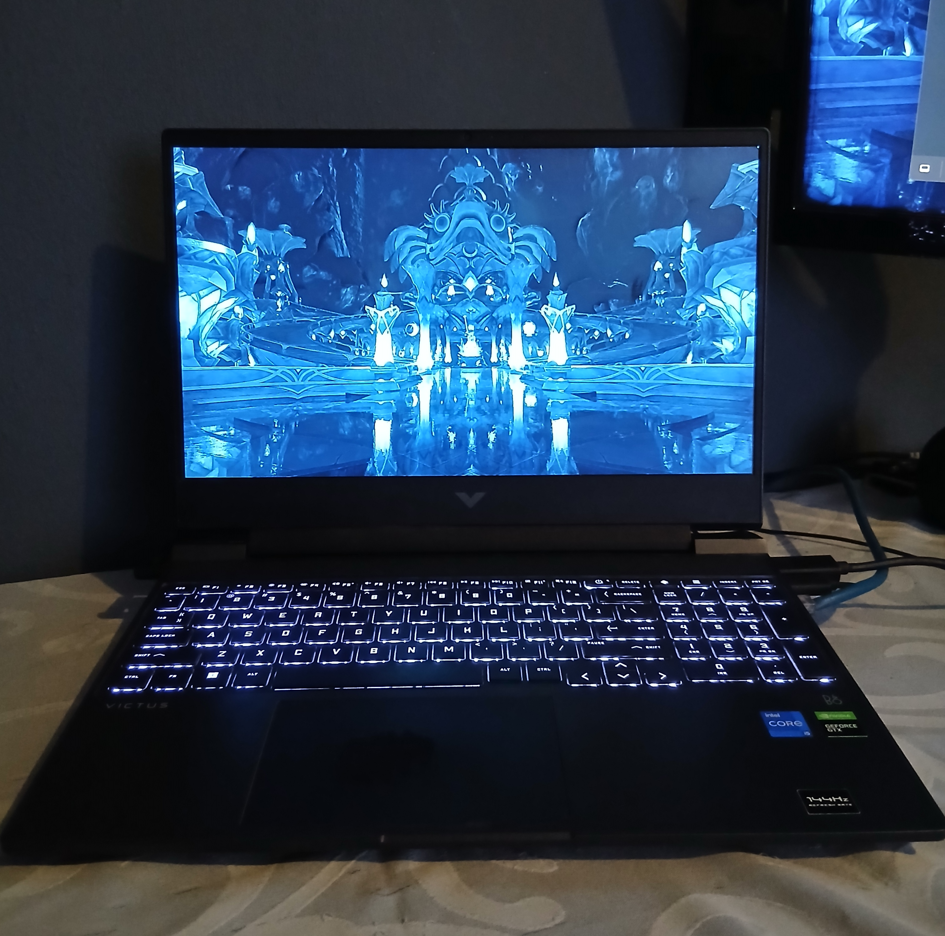
\includegraphics[width=0.8\textwidth]{pc.png} % Asegúrate de que 'pc.jpg' esté en la misma carpeta o especifica la ruta
    \caption{Ordenador portátil HP Victus utilizado para el desarrollo y pruebas del sistema.}
    \label{fig:hp_victus}
\end{figure}

El uso de este equipo demostró que, gracias a la contenedorización, es posible simular y desarrollar para sistemas distribuidos complejos sin la necesidad inmediata de una infraestructura de hardware a gran escala, validando la portabilidad y eficiencia del software desarrollado.

\subsection{Software Utilizado}
La selección del software se centró en tecnologías modernas, de código abierto y alineadas con los requerimientos de un sistema distribuido, asíncrono y portable.

\begin{itemize}
    \item \textbf{Visual Studio Code:} Fue el entorno de desarrollo integrado (IDE) principal para la escritura y depuración del código. Su naturaleza ligera, junto con un potente ecosistema de extensiones, lo convirtieron en la herramienta ideal. Se utilizaron extensiones clave para el desarrollo con Python (ofreciendo autocompletado, \textit{linting} y formato de código) y para la integración con Docker, que permitió gestionar los contenedores, visualizar sus estados y acceder a sus registros directamente desde el editor.

    \item \textbf{Python 3.12:} Fue el lenguaje de programación elegido para desarrollar el servicio \textit{Nez-Daemon Watcher}. Su elección se justifica por su robusto soporte para la programación asíncrona a través de la biblioteca \texttt{asyncio}, fundamental para gestionar operaciones de red y de sistema de archivos de manera concurrente y eficiente. Además, se utilizó un ecosistema de librerías clave, entre las que destacan:
    \begin{itemize}
        \item \texttt{watchdog}: Para el monitoreo continuo y no bloqueante del sistema de archivos.
        \item \texttt{httpx}: Un cliente HTTP asíncrono moderno, utilizado para la comunicación resiliente con la API REST del \textit{Router} de MictlanX.
        \item \texttt{python-dotenv}: Para la gestión de la configuración a través de variables de entorno, adhiriéndose a los principios de la metodología \textit{12-Factor App}.
    \end{itemize}
    
    \item \textbf{Docker:} Es una pieza central de la arquitectura. Se utilizó para empaquetar el \textit{Nez-Daemon Watcher} y todas sus dependencias en una imagen de contenedor portátil. Asimismo, se empleó para desplegar el ecosistema completo de MictlanX en el entorno de desarrollo. El uso de Docker garantiza la consistencia entre los entornos de desarrollo y producción, simplifica el despliegue y aísla los servicios, cumpliendo con el requerimiento no funcional de portabilidad.

\item \textbf{MictlanX Virtual Storage Space (VSS):} Actuó como el sistema de almacenamiento distribuido de destino. Para las pruebas, una instancia completa del VSS, incluyendo su \textit{Router} y múltiples nodos \textit{Peer}, fue desplegada localmente mediante contenedores Docker. Esto permitió validar la correcta interacción del \textit{Watcher} con la API de MictlanX para la subida, replicación y verificación de archivos.
\end{itemize}

\subsection{Elementos a Evaluar}

Durante las fases de desarrollo y pruebas se evaluó la funcionalidad del cliente implementado en C++. El análisis se centró en verificar su comportamiento al interactuar con los datos alojados en el Espacio de Almacenamiento Virtual (VSS) de MictlanX, así como en revisar que cumpliera adecuadamente con las operaciones previstas dentro del flujo de trabajo.

Se comprobó que el cliente permite consultar archivos individuales y también manejar estructuras más amplias, como carpetas completas que contienen expedientes de pacientes. Esto facilitó revisar distintos escenarios de uso y confirmar que el sistema es capaz de procesar información en diferentes niveles de organización.

También se evaluaron las operaciones básicas de transferencia de datos, incluyendo la subida y descarga de archivos hacia y desde la nube. Estas pruebas se realizaron para identificar posibles fallos, validar el manejo de errores y asegurar que la información pudiera ser transferida sin modificaciones no deseadas.

Hasta ahora los resultados obtenidos permitieron identificar el comportamiento del cliente bajo condiciones de uso típicas y detectar áreas donde podrían requerirse ajustes o mejoras en futuras iteraciones del sistema.

\newpage

\subsection{Pruebas}
La validación del sistema se realizo en dos fases principales. La primera se enfoco en evaluar el servicio \textit{Watcher} de forma aislada, mientras que la segunda consistio en revisar su funcionamiento al integrarse con los componentes responsables de la comunicacion externa.
En la fase inicial, el \textit{Watcher} se probo de manera independiente con el proposito de confirmar su funcion principal: detectar nuevos archivos y enviarlos automaticamente al VSS de MictlanX. Para ello, el servicio se ejecuto dentro de un contenedor Docker con el fin de contar con un entorno controlado y reproducible durante las pruebas. 

La supervisacion del comportamiento en tiempo real se realizo mediante el comando \texttt{docker logs -f <container\_id>}, lo cual permitio observar la secuencia de eventos desde la deteccion de un archivo hasta la confirmacion de su carga.

El analisis de estas trazas facilito la identificacion de fallos y la revision del flujo interno del servicio. Entre los problemas detectados se encontraron errores de conexion con la API de MictlanX, interrupciones temporales en las solicitudes y comportamientos inesperados asociados con la logica de reintentos. Esta informacion permitio ajustar la implementacion y verificar que las correcciones aplicadas resolvieran los incidentes sin generar efectos secundarios.

\begin{figure}[h!]
    \centering
    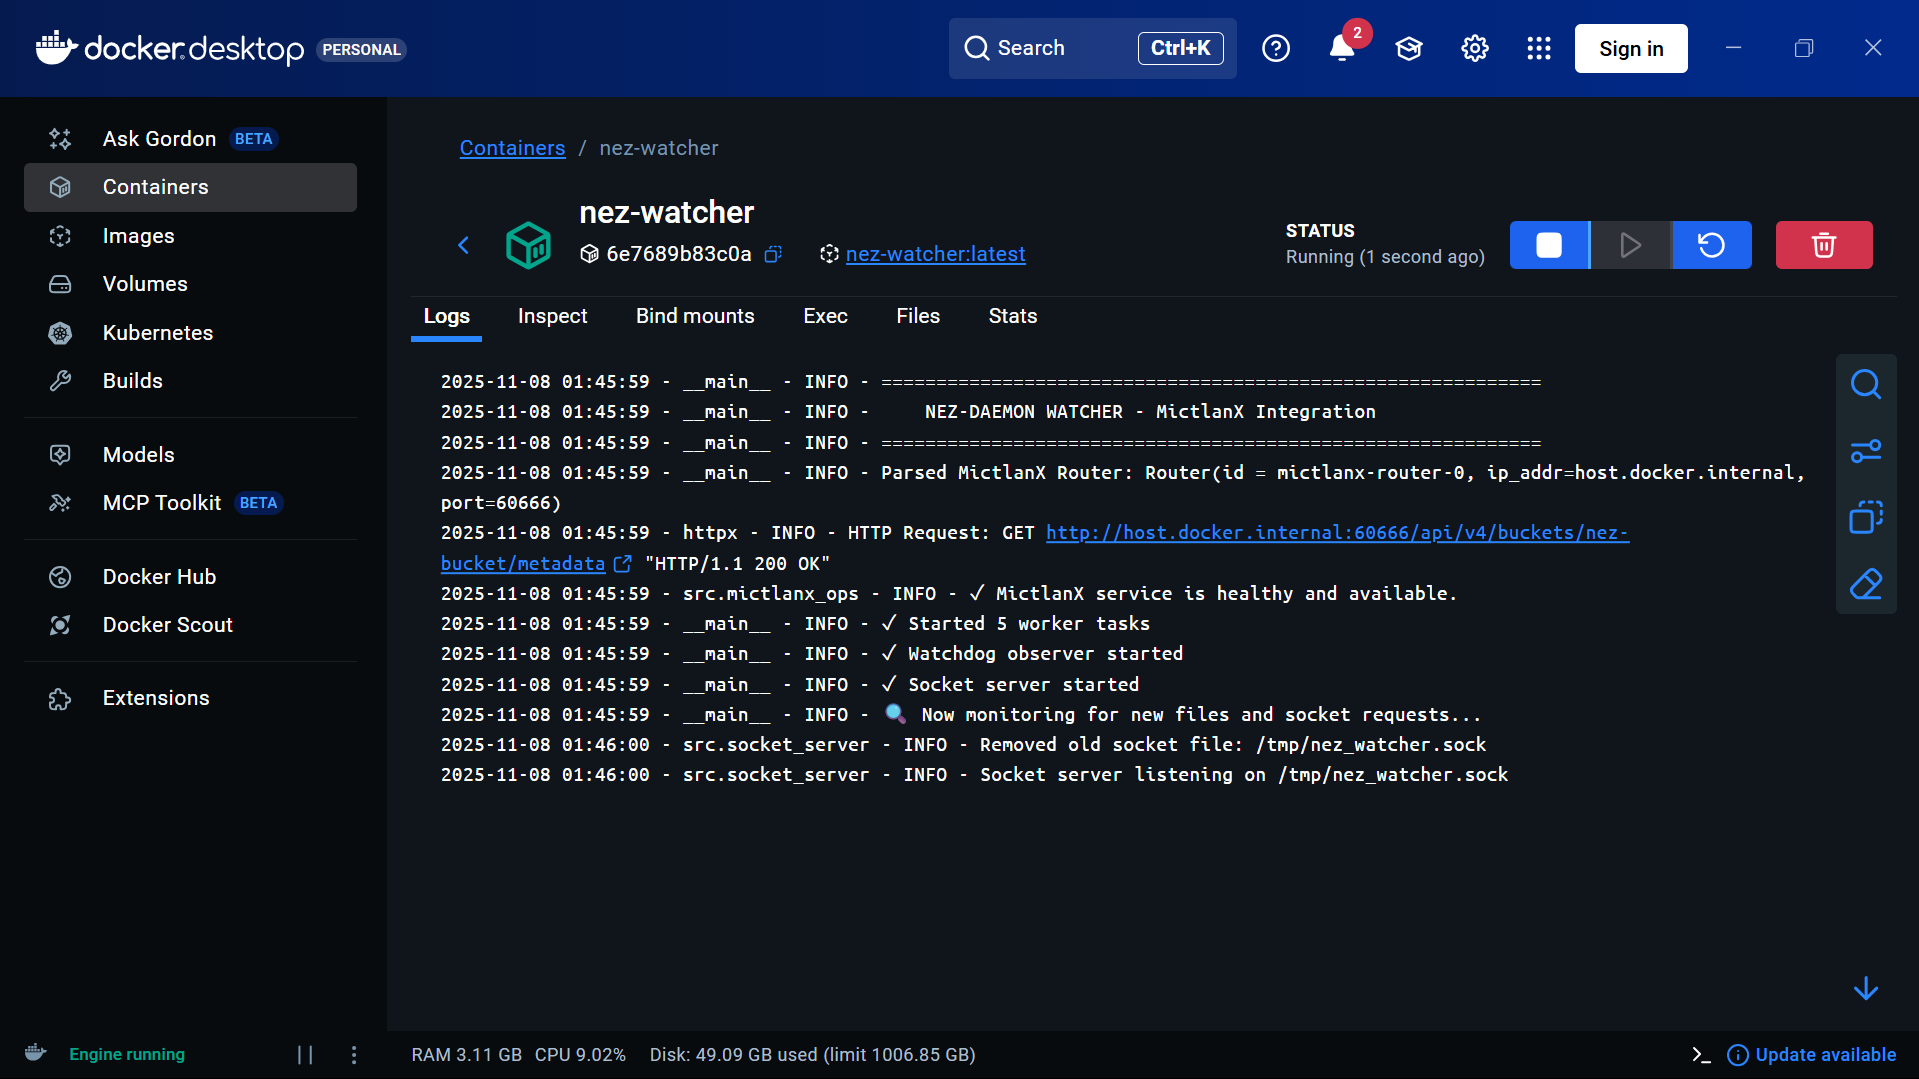
\includegraphics[width=\textwidth]{Diagramas UML/ss_inicio.png} % Reemplazar con la imagen de los logs
    \caption{Captura de los registros al iniciar el servcio}
    \label{fig:watcher_logs}
\end{figure}

Una vez validado el flujo de carga, las pruebas se extendieron a los mecanismos de comunicación para la descarga de archivos. Se probó de manera exhaustiva el socket de dominio Unix, confirmando que el \textit{Watcher} podía recibir y procesar peticiones de otros procesos locales. Posteriormente, se integró el cliente desarrollado en C++ a este flujo. El objetivo era simular el caso de uso completo en el que una aplicación externa (el cliente) solicita la descarga de un archivo o expediente a través del socket. El éxito de estas pruebas confirmó que el \textit{Watcher} no solo actúa como un agente de ingesta, sino también como una puerta de enlace funcional para que otras partes del sistema accedan a los datos almacenados en MictlanX, preparándolo para su integración en un flujo de trabajo o \textit{deployer} más amplio.
